%==============================================================================
% Matt Nichols' Homework Template
%==============================================================================


%Fill out this line with the homework number
\newcommand{\visibleusernames}
{\space man1, malesser, ac110 }
{}
\newcommand{\thisclass}{CSCI 160}
\newcommand{\thishw}{Final Project}

%==============================================================================
% Formatting parameters
%==============================================================================

\documentclass[11pt]{article}			% 11pt article
\author{Matt Nichols}
\date{\today}
\makeatletter					% Make '@' accessible.

%Fill out this line with your name and login
\def\@oddhead{\bf \thisclass \space - \thishw\hfill \visibleusernames} % Here they are

\oddsidemargin=0in				% Left margin minus 1 inch.
\evensidemargin=0in				% Same for even-numbered pages.
\textwidth=6.5in				% Text width (8.5in - margins).
\topmargin=0in					% Top margin minus 1 inch.
\headsep=0.2in					% Distance from header to body.
\textheight=8.5in					% Body height (incl. footnotes)
\skip\footins=4ex				% Space above first footnote.
\hbadness=10000					% No "underfull hbox" messages.
\makeatother					% Make '@' special again.

%==============================================================================
% Packages used
%==============================================================================

\usepackage{amsmath}				% want AMS fonts
\usepackage{amssymb}
%\usepackage{psfig}				% want to include EPS files
\usepackage[pdftex]{graphicx}				% for including images
\usepackage{algorithmic}
\usepackage{algorithm}
\usepackage{hyperref}
\usepackage{tikz}


%==============================================================================
% Macros
%==============================================================================
\newcommand{\new}[1]{{\em #1\/}}		% New term (set in italics).
\newcommand{\set}[1]{\{#1\}}			% Set (as in \set{1,2,3})
\newcommand{\setof}[2]{\{\,{#1} $\mid$~{#2}\,\}}	% Set (as in \setof{x}{x > 0})
\newcommand{\N}{\mathord{\Bbb N}}		% Positive integers.
\newcommand{\compl}[1]{\overline{#1}}		% Complement of ...            
\newcommand{\bigand}{\bigwedge}
\newcommand{\bigor}{\bigvee}
\newcommand{\OR}{\vee}
\newcommand{\AND}{\wedge}
\newcommand{\code}[1]{\texttt{#1}}
\newcommand{\nlogn}{n \log n}

\newcounter{qcounter}
\setcounter{section}{0}
\def\thesection{Section \arabic{section}}


% \begin{list}{b\alph{qcounter}.}{\usecounter{qcounter}} <-- helpful

%==============================================================================
% Title
%==============================================================================

\begin{document}
\centerline{\bf \LARGE\thishw: Knock Detection Entry System}
\centerline{\today}

\section{Introduction}
 % Introduce your project. Succinctly explain your problem and solution. Why did you choose to work on it?
Carrying keys around has always been a hassle for all of us. If one loses a key, he or she has to be assisted by someone else to get in to the room. A lot of times, there are situations where you wouldn't want to bring your keys with you either, such as when you're going on a run.I personally have forgotten my keys in my room, or have been locked out by my roommate numerous times. We wanted an easier way to enter and exit a locked room, and not ever have to worry about being locked out. 
Our project is a reasonably straightforward Arduino program which enables pulling a doorhandle down from the inside of a door once a specific pattern of knocks has been detected. This pattern is configurable via a "record" function, and, when powered, the device is always listening for the pattern, ready to trigger a motor to open the door. If an incorrect knock pattern is given, the program alerts you through a buzz in the speaker. This way, the room is secure and you'll never be locked out because you don't have the key.

\section{Architecture}
% Describe the architecture of your system. Figures are welcomed and encouraged


\begin{center}
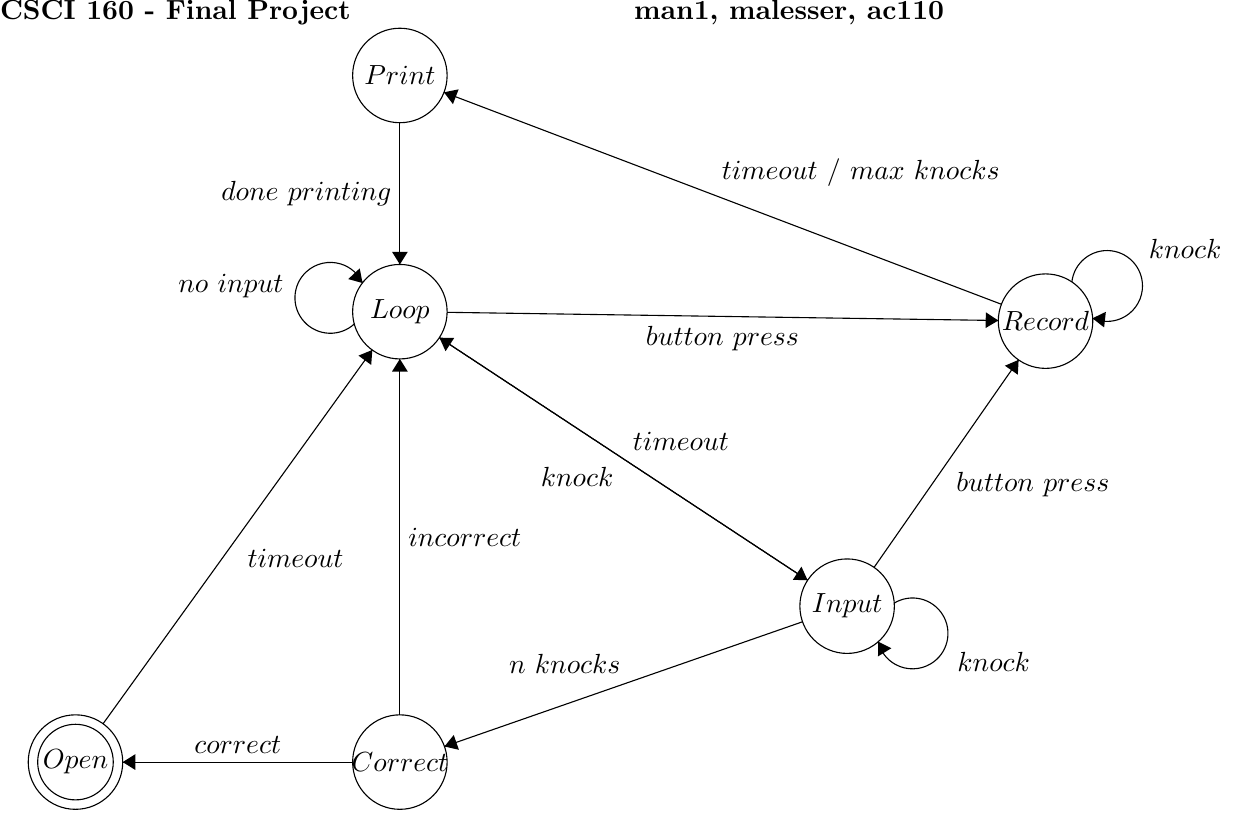
\begin{tikzpicture}[scale=0.2]
\tikzstyle{every node}+=[inner sep=0pt]
\draw [black] (26.6,-22.6) circle (3);
\draw (26.6,-22.6) node {$Loop$};
\draw [black] (55,-41.3) circle (3);
\draw (55,-41.3) node {$Input$};
\draw [black] (67.6,-23.2) circle (3);
\draw (67.6,-23.2) node {$Record$};
\draw [black] (26.6,-51.2) circle (3);
\draw (26.6,-51.2) node {$Correct$};
\draw [black] (6,-51.2) circle (3);
\draw (6,-51.2) node {$Open$};
\draw [black] (6,-51.2) circle (2.4);
\draw [black] (26.6,-7.6) circle (3);
\draw (26.6,-7.6) node {$Print$};
\draw [black] (29.6,-22.64) -- (64.6,-23.16);
\fill [black] (64.6,-23.16) -- (63.81,-22.64) -- (63.79,-23.64);
\draw (47.08,-23.48) node [below] {$button\mbox{ }press$};
\draw [black] (29.11,-24.25) -- (52.49,-39.65);
\fill [black] (52.49,-39.65) -- (52.1,-38.79) -- (51.55,-39.63);
\draw (37.85,-32.45) node [below] {$knock$};
\draw [black] (23.713,-23.373) arc (312.7283:24.7283:2.25);
\draw (19.24,-20.97) node [left] {$no\mbox{ }input$};
\fill [black] (24.23,-20.78) -- (24.05,-19.85) -- (23.32,-20.53);
\draw [black] (52.49,-39.65) -- (29.11,-24.25);
\fill [black] (29.11,-24.25) -- (29.5,-25.11) -- (30.05,-24.27);
\draw (44.45,-31.45) node [above] {$timeout$};
\draw [black] (52.17,-42.29) -- (29.43,-50.21);
\fill [black] (29.43,-50.21) -- (30.35,-50.42) -- (30.02,-49.48);
\draw (37.07,-45.62) node [above] {$n\mbox{ }knocks$};
\draw [black] (23.6,-51.2) -- (9,-51.2);
\fill [black] (9,-51.2) -- (9.8,-51.7) -- (9.8,-50.7);
\draw (16.3,-50.7) node [above] {$correct$};
\draw [black] (57.982,-41.109) arc (121.40093:-166.59907:2.25);
\draw (61.97,-44.82) node [right] {$knock$};
\fill [black] (56.97,-43.55) -- (56.96,-44.49) -- (57.81,-43.97);
\draw [black] (26.6,-48.2) -- (26.6,-25.6);
\fill [black] (26.6,-25.6) -- (26.1,-26.4) -- (27.1,-26.4);
\draw (27.1,-36.9) node [right] {$incorrect$};
\draw [black] (7.75,-48.77) -- (24.85,-25.03);
\fill [black] (24.85,-25.03) -- (23.97,-25.39) -- (24.78,-25.98);
\draw (16.89,-38.28) node [right] {$timeout$};
\draw [black] (64.8,-22.13) -- (29.4,-8.67);
\fill [black] (29.4,-8.67) -- (29.97,-9.42) -- (30.33,-8.48);
\draw (55.86,-14.69) node [above] {$timeout\mbox{ }/\mbox{ }max\mbox{ }knocks$};
\draw [black] (26.6,-10.6) -- (26.6,-19.6);
\fill [black] (26.6,-19.6) -- (27.1,-18.8) -- (26.1,-18.8);
\draw (26.1,-15.1) node [left] {$done\mbox{ }printing$};
\draw [black] (69.27,-20.722) arc (173.74488:-114.25512:2.25);
\draw (74.12,-18.63) node [right] {$knock$};
\fill [black] (70.58,-23.02) -- (71.32,-23.6) -- (71.43,-22.61);
\draw [black] (56.71,-38.84) -- (65.89,-25.66);
\fill [black] (65.89,-25.66) -- (65.02,-26.03) -- (65.84,-26.6);
\draw (61.9,-33.61) node [right] {$button\mbox{ }press$};
\end{tikzpicture}
\end{center}


\section{Implementation}
% Challenges, etc.

\section{Evaluation}
% did it work? Are there any corner cases? How would you solve them?
Yes it did work. 

\section{Related Work}
% Are there any similar solutions? Compare yours to theirs, if possible.
There aren't many similar affordabe solutions. Doors with fingerprint scanners exist but are extremely expensive, even though they're more secure. These go for around \$300.

"The Clapper" also exists, that gives current to an outlet if it detects claps. However, it doesn't let you customize the sequence of claps. It doesn't directly connect to a motor either. Lastly, it detects sound as a pose to vibrations. Our project won't detect random noises, only vibrations on the door whereas "The Clapper" could interpret white noise and randomly open and close the door. "The Clapper" goes for around \$20. 
\includegraphics[scale=0.75]{theclapper.jpg}

Lockitron is a kickstart that uses smart phones to lock and unlock doors. To use lockitron, you first need to attach the lockitron shell around your deadbolt. This shell is smart; it's connected to wifi and has bluetooth. From anywhere in the world, you can unlock or lock your door from your smartphone. You can also grant access to other users. Lockitron also automatically unlocks the door when you walk near it with your smartphone. With lockitron, you would still either need your key or a phone to get into you're locked house. It doesn't entirely address the problem we were having. You can still lock your phone inside the house, and if you don't want to run with keys, why would you run with your phone. We need a solution that doesn't physically require any hardware, and lockitron doesn't give us that. It also costs around \$200.
\url{https://lockitron.com/preorder}

Our project's cost came out to around \$50. If we were to sell this project, our costs would decrease of bulk order so we could sell for around \$70.

\section{Future Work}
% Describe here features that you wanted to implement, but due to time/resource constraints you weren't able to.

In the remote\_unlock/ directory of the repo, we have the backend/server script for implementing SMS-triggered unlocking as well (via Twilio). Alas, we haven't yet had any successes in configuring the device's side of this functionality; however, should the device be configured with an ethernet shield, it would be simple to poll against [server port]/state and trigger the servo when the "Unlocked" state is observed.

\end{document}